\documentclass[12pt,a4paper]{scrartcl}

\usepackage[ngerman]{babel} % use German descriptions like Abbildung, Tabelle, ...
%\usepackage[english]{babel} % use English descriptions like figure, table, ...
\usepackage[utf8]{inputenc} % important for character encoding to use utf-8 allows special chars
\usepackage[T1]{fontenc}    % set font

\usepackage[hypcap=false]{caption}

\usepackage[osf]{mathpazo} 
\linespread{1.05}\selectfont 
\usepackage{booktabs}
\usepackage{tabularx}
\usepackage{hyperref}
\usepackage{amsmath}
\usepackage{amsfonts}
\usepackage{amssymb}
\usepackage{lmodern}
\usepackage{graphicx}
\usepackage{lipsum}
\usepackage{hyperref}
\usepackage{enumitem}
\usepackage[dvipsnames]{xcolor}
\usepackage{framed} 
\usepackage{url}
\usepackage[font={footnotesize,it}]{caption}

\setlength\parindent{0pt} 


%---------------------------------------
% SETUP der Bilder
%---------------------------------------


%---------------------------------------
% SETUP der Kursinformationen
%---------------------------------------
\newcommand{\myLecture}{Human Computer \newline Interaction}
\newcommand{\mySemester}{WS2023/2024}
\newcommand{\myTeacher}{Prof. Ute Trapp}

%\newcommand{\mySupervisor}{Ute trapp}

%---------------------------------------
% SETUP der Praktikumsinformationen
%---------------------------------------
\newcommand{\myPractical}{Praktikum 1}         % BEI JEDEM TERMIN ANPASSEN
\newcommand{\myDate}{\today}


\newcommand{\myStudentOne}{Abdullah & & }
\newcommand{\myStudentTwo}{Anton & & }
\newcommand{\myStudentThree}{Bogdan & & }
\newcommand{\myStudentFour}{Días & & }



\newcommand{\myStudentsTable}{
\begin{tabular}{rcll}
    \toprule
    \textbf{Datum:}          & \myDate       & & \\ 
   % \textbf{Aufsicht:}    & \mySupervisor \\
    \textbf{Studenten:}      & \myStudentOne     \\
                            & \myStudentTwo     \\
                            & \myStudentThree     \\ 
                            & \myStudentFour     \\ 
    \bottomrule
\end{tabular}     
}

\def\code#1{\texttt{#1}}


\begin{document}

%---------------------------------------
\begin{minipage}{\linewidth}

    \begin{minipage}{.7\linewidth}
        \textbf{\Huge \myLecture~--~\mySemester\vspace{.5em}}\\
        {\large ~~by \myTeacher\vspace{1em}}\\
    \end{minipage}
    
    \begin{minipage}[t]{.3\linewidth}
        \centering
        
\includegraphics[width=\linewidth]{images/hda-blue.pdf}
    \end{minipage}\\
    
    \begin{minipage}{\linewidth}
    \begin{center}
        \textbf{\myPractical}\vspace{.5em}\\
        \myStudentsTable
    \end{center}
    \end{minipage}
\end{minipage}
%---------------------------------------

\tableofcontents	 		%Inhaltsverzeichnis
\newpage

\section{Agiles framework}

Als Auswahl stehen viele Verschiedene Vorgehensmodelle, welche die Arbeit am Projekt eines Teams auf verschiedene Art und Weise leiten. In der Vorlesungen am \code{26.10.2023} wurden einige Frameworks detailierter analysiert. Dies waren:
\begin{itemize}
\item Double Diamond

\item Lean UX

\item Agile UX

\item Design Sprint
\end{itemize}
Jedes dieser Frameworks hat natürlich seine Vor- und Nachteile. Letztendlich hat sich die Gruppe für ein Franework entschieden.

\subsection{Warum Agile UX?}

\subsubsection{Was ist Agile UX}

Agile UX ist ein relativ neues Vorgehensmodell, wie ein Team an einem Projekt arbeitet. Es hat 5 Kernprinzipien:
\begin{enumerate}
\item \textbf{Inkrementelle Entwicklung und "bite-sized" Lieferung}\\
Wie alle agilen Vorgehensmodelle ist die Ideee bei $Agile UX$ das Produkt nicht mit einem "Big-Bang" am Ende der 	Vorgegebenen Zeit vollständig zu liefern, sondern Iterativ in kleinen Schritten. Ziel dabei ist es immer ein MVP(\textbf{M}inimal \textbf{V}iable \textbf{P}roduct) zu liefern.
\begin{figure}[h]
    \centering
    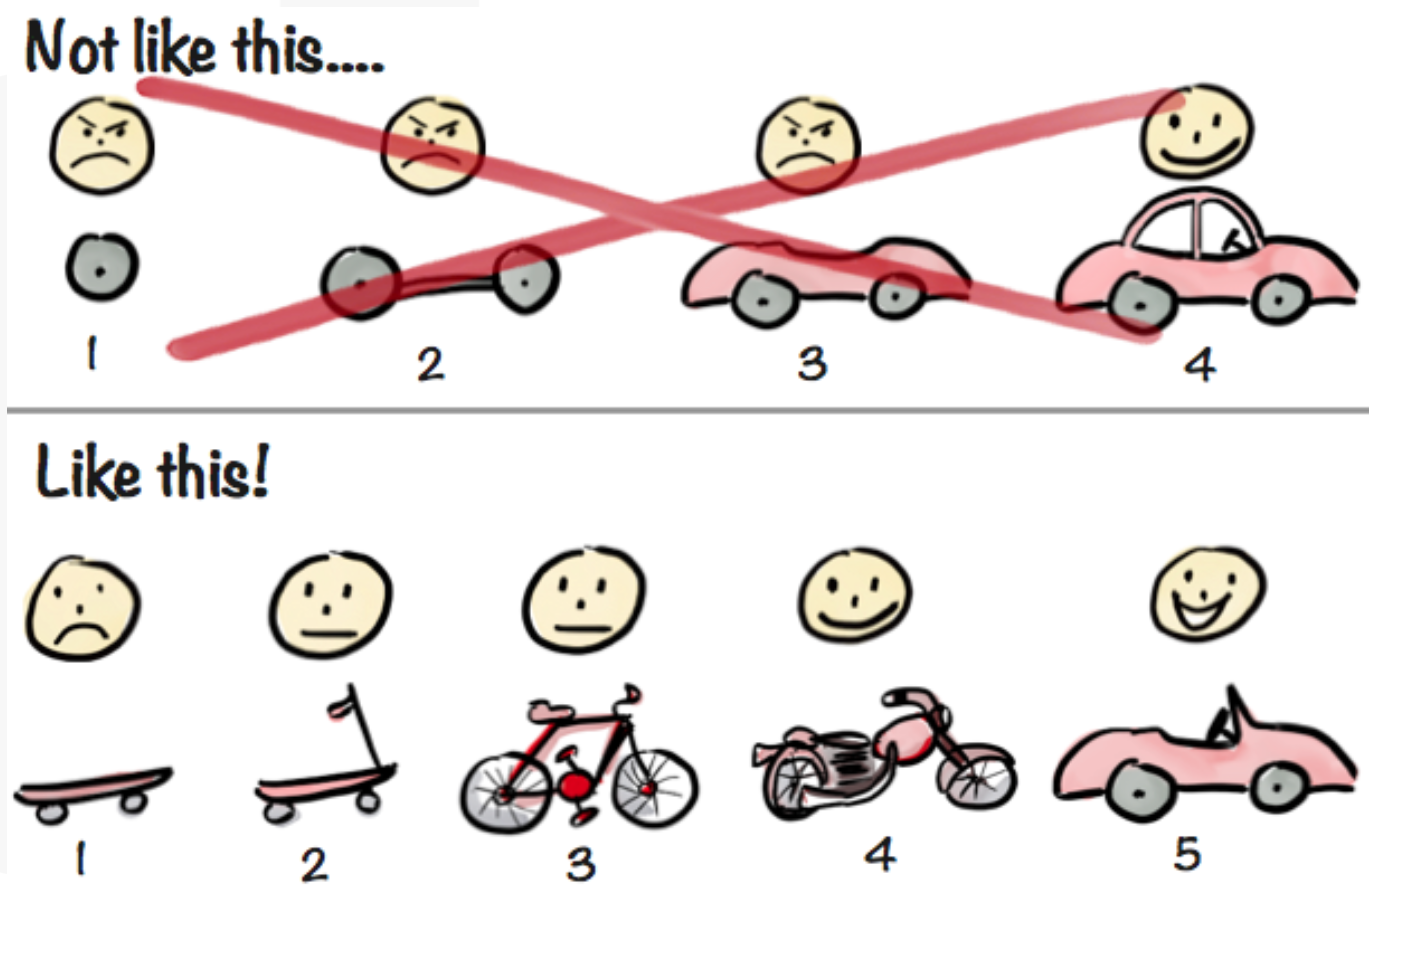
\includegraphics[width=0.5\textwidth]{images/IterativesVorgehen}
    \caption{Bild: Not like this. . . by Henrik Kniberg: \url{blog.crisp.se}}
\end{figure}

\item \textbf{Flexibiltät und Adaptivität}\\
Designer und Entwickler müssen auf sich ändernde Anforderungen anpassen können. Deshalb wird das Vorgehen auch "agil" genannt.

\item \textbf{Kollaboration und Kommunikation}\\
Es ist ständig Kommunikation gefprdert, nicht nur unter den Entwicklern, sondern auch mit Stakeholdern und Nutzern

\item \textbf{Eingespieltes Team}\\
Die Entwickler müssen zusammen in den sprints als Teams arbeiten. Die Teams müssen kreativ, schnell und anderen Teammitgliedern rechenschaftspflichtig sein.

\item \textbf{Nutzer-Feedback}\\
Das $UX$ in $Agile UX$ steht für "User Experience". Das heißt, dass der Kunde in den Entwicklungsprozess mehr eingebunden wird. Dieser kann kontinuierlich Feedback geben bezüglich des Zwischenstands des Projekts. Dadurch stellt man sicher, dass der Kunde das bekommt, was er Erwartet und die Entwickler wissen besser, was von ihnen erwartet wird. 
\end{enumerate}

\begin{figure}[h]
    \centering
    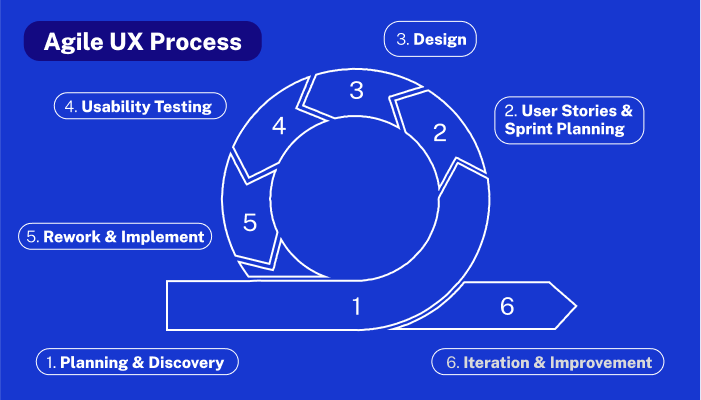
\includegraphics[width=0.8\textwidth]{images/AgileUX}
    \caption[Abbildung: Agile UX Vorgehen]{Das Agile UX Vorgehensmodell}
    \footnote{UX Vorgehensmodell \url{https://www.linkedin.com/pulse/agile-ux-intersection-user-experience-development-door3/}}
    
\end{figure}


\subsubsection{Gründe für Agile UX}

$Agile UX$ bietet sich aus dem Grund besonders gut für unser Projekt, wegen den Schnellen Iterationen. Die Empfohlene Sprint-Dauer von 2 Wochen passt gut in den Praktikumszyklus.   Das regelmäßige Abholen von Feedback vom Kunden ist in einem Projekt wie diesem, wo man viel an der UI arbeitet sehr weiterhelfend. Das sich ein Kunde sich nicht mit dem Code beschäftigt sondern eher mit der UI, kriegt man auch hauptsächlich Feedback zur UI. \\
Agile UX ist ein kompliziertes Vorgehensmodell, weshalb es in Unternehmen bis jetzt nicht oft verwendet wird, wir arbeiten jedoch in einer kleinen Gruppe von 4 und können uns daher effizient miteinander kommunizieren und koordinieren. \\
Wir erwarten, dass es sehr schwer sein wird, die Agile UX straffen Zeitpläne einzuhalten, wir derden es aber bestmöglich versuchen einzuhalten :)


\section{Vision}

\subsection{Entscheidungsprozess}

Zunächst hatten wir einige Projektideen in der Gruppe gesammelt. Über einige Tage hinweg sammelten wir folgende Vorschläge:
\begin{itemize}
\item To-Do App

\item live Währung-Umrechner

\item Wetter-App

\item Rezepte-App

\item Snake-Spiel

\item Ernährungs-Planer

\item [\dots]
\end{itemize}

Letztendlich entschieden wir uns für eine Wetter-App, da es uns am interessantesten erschien und am Meisten Potential drin gesehen habe.

\subsection{Projektvision}

Viele Menschen, die an verschiedenen Tagen verschieden viele Informationen zum Wetter brauchen haben zwei oder mehr Wetter-Apps auf dem Handy, um alle Situationen abzudecken: \\
Eine minimalistische Wetter-App, in der man schnell die Temperatur sieht und ob es regnen wird oder nicht. Eine zweite für eine besondere nieschige Metrik, die es in der Standart Wetter App nicht gibt. Beispielsweise müssen Surfer wissen in welche Richtung der Wind wie stark wehen wird. \\
Wir planen also eine Wetter-App zu erstellen, welche einen minimalistischen Modus hat und einen einstellbaren Detail-Modus, wo man die Metriken, die man braucht auch einstellen kann. Dadurch können wir eine Wetter App "für alle" erstellen, sodass niemand mehr zwei Wetter-Apps auf dem Handy haben muss.\\

Außerdem planen wir die Anwendung nicht als eine reine Wetter-App zu lassen. Eine Idee ist es, einen Kalender in die App einzubauen. Über einen Link (wie der im OBS) kann man dann Termine eintragen lassen. Dadurch kann die App dem Nutzer mitteilen, ob er für den Hin- oder Rückweg einen Regenschirm braucht, eine Empfehlung geben wie viele Schichten an Kleidung der Nutzer anzeihen soll usw. \dots 

\section{User Research}
\subsection{Benutzer und Kriterien definieren}

Wie bereits in dem Kapitel "Projektvision" erwähnt planen wir eine App für alle zu designen. Daher müssen die Verschiedensten Kundengruppen. Es hat jeder, der ein Handy hat, eine Wetter-App. In Deutschland sind es $67,6$ Millionen Menschen, damit sind es $81,25\%$ der Bevölkerung, die  Nutzer sind. \\
Hauptsächlich sind es aber Menschen, die viel Zeit draußen verbringen (müssen), outdoor-Sportler oder Pendler. 

\subsection{Nutzer analysieren}
TODO


\subsection{Benutzergruppen definieren}
TODO

\subsection{Stereotypen festlegen}
TODO

\subsection{stereotyp-Beschreibung}
TODO

\subsection{Teilstandardisierte Interview}
TODO

\subsection{Anwendungsszenarien}
TODO

\subsection{Anforderungen + Use Cases}
TODO



%---------------------------------------
% Ende
%---------------------------------------
\end{document}